\documentclass[11pt]{article}
\usepackage{icmlko}
\begin{document}

\title{바닥 아래에는 신호가 없다 --- 세계애니를 넓힐 수 없는 이유}
\author{월드모델 실험실}
\date{노트 376 · 2026년 8월 1일}
\maketitle

\begin{abstract}
노트 375가 세계애니를 판에서 제일 심하게 잘린 도메인으로 짚었다 ---
popularity 최소 19,533 · 중앙 49,618. 가중 10\% · 유보 300행이라 넓히면
판이 크게 움직인다. \textbf{넓힐 수 있는지 먼저 쟀다.} 노트 372가 만든
절차 그대로 --- AniList 인기 순위 3,001위 아래를 1,181편 받아 2025년 이후
99편을 \emph{유보에만} 넣고, 학습은 그대로 둔 채 한 번의 적합 안에서
위/아래를 갈랐다.

\textbf{바닥 위 $+0.5573$ 대 바닥 아래 $\mathbf{+0.0223}$}(같은 크기
무작위 대비 $p=1.000$). 그런데 아래쪽은 라벨 퍼짐이 0.086 로 위쪽(0.261)의
3분의 1이라 \emph{좁아서 낮은 것}일 수 있다 --- 사전 등록에 그 실패를 적어
뒀다. 그래서 위쪽에서 \textbf{같은 퍼짐(SD 0.086)의 연속 99행}을 잘라
견줬다: \textbf{$+0.3660$}. \textbf{퍼짐이 같은데 위는 되고 아래는 안 된다
--- 범위 문제가 아니라 신호가 없다.}

안 넓힌다. 그리고 ``두 모집단이 안 섞인다''가 \textbf{세 종류}가 됐다:
\emph{수준형}(노트 353 · 357 --- 기준 안에서는 멀쩡, 따로 재면 쓴다) ·
\emph{부호형}(노트 372 --- 따로 재도 음수) · \emph{무신호형}(노트 360 ·
376 --- 따로 재면 0). 뒤의 둘은 못 쓴다.
\end{abstract}

\section{절차는 노트 372의 것}

노트 372가 만화 KR 에서 쓴 설계를 그대로 옮겼다 --- \textbf{학습을
건드리지 않고} 새 행을 유보에만 넣어 \emph{한 번의 적합 안에서} 부분집합끼리
견준다(노트 371이 그은 경계).

AniList \texttt{media(type: ANIME, sort: POPULARITY\_DESC)} 의 61쪽부터
받아 1,181편을 얻었다 --- popularity 10,298\textasciitilde{}19,530 으로
\textbf{기존 바닥 19,533 과 정확히 이어진다}(기존 세트가 인기 상위
$\sim$3,000편이라는 노트 375의 추론이 여기서 확인된다). 그중 2025년 이후
99편을 유보에 넣었다(유보 $300 \to 399$, 학습 2,648 그대로).

\textbf{옛 행이 안 움직이는지 먼저 봤다}(사전 등록 위험). 축 다섯 중 넷은
100\% 그대로이고 \texttt{venue\_prominence} 만 98.6\% 그대로다(제작사 사전
작품 수라 표본에 따라 조금 움직인다, 평균 $|$차$|$ 0.0006). 라벨은 100\%
그대로다.

\section{아래는 0 이다}

\begin{center}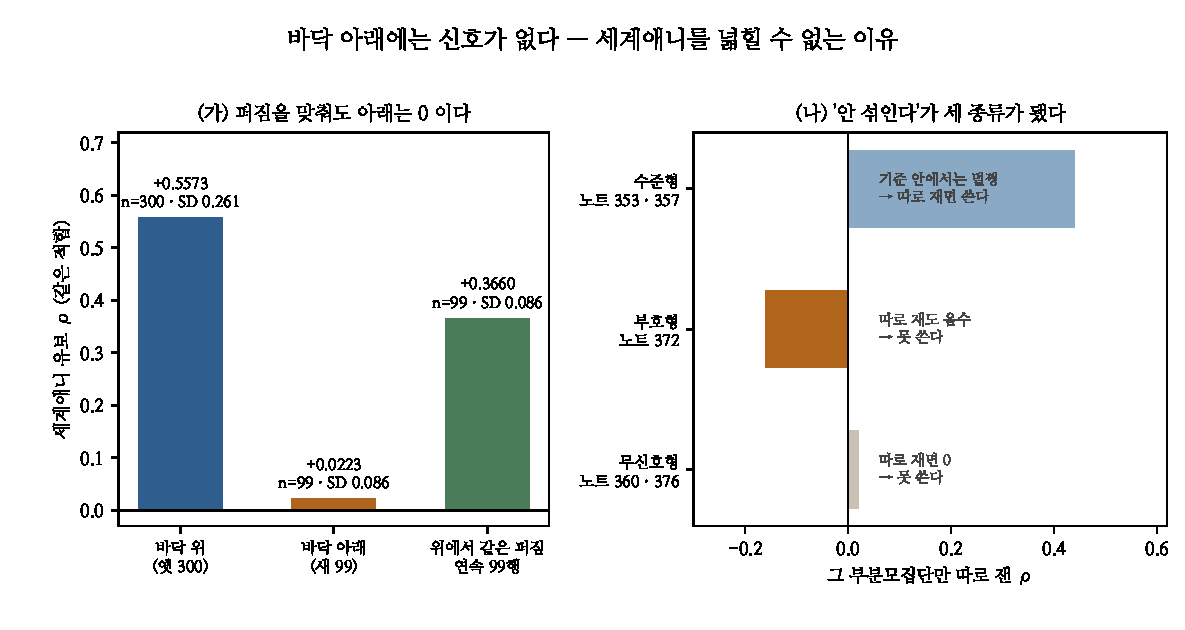
\includegraphics[width=\linewidth]{figs/below.pdf}\end{center}

\begin{center}
\begin{tabular}{lrrl}
\hline
부분집합 & $n$ & $\rho$ & 같은 크기 무작위 \\
\hline
바닥 위(옛) & 300 & $+0.5573$ & $+0.5580$ (SD 0.023) $p=0.530$ \\
\textbf{바닥 아래(새)} & 99 & $\mathbf{+0.0223}$ & $+0.5541$ (SD 0.068) $p=1.000$ \\
전부 & 399 & $+0.5584$ & --- \\
\hline
\end{tabular}
\end{center}

\textbf{섞어도 판이 안 움직인다}($0.5567 \to 0.5584$) --- 99행이 399행 중
4분의 1이고 무리 사이 순위가 그만큼 벌어 주기 때문이다(무리 안으로 다시
매기면 $+0.4246$). \textbf{점수가 안 내려간다고 넣어도 되는 게 아니다.}

\section{좁아서인가, 없어서인가}

사전 등록에 적어 뒀다: \emph{아래쪽은 라벨 범위가 좁다. 범위가 좁으면
스피어만이 낮게 나오는 것이 당연하다 --- 같은 크기 · 같은 퍼짐 부분집합과
견준다.}

라벨 퍼짐(log10)이 위 $0.261$ 대 아래 $\mathbf{0.086}$ 이다. 무작위
부분집합으로는 그 퍼짐을 못 만든다(넓은 집합에서 99개를 뽑으면 SD 0.214가
한계였다). 그래서 \textbf{위쪽을 라벨 순으로 정렬해 연속 99행}을 잘랐다 ---
퍼짐이 정확히 0.086 이 되는 창이다.

\begin{center}
\begin{tabular}{lrrr}
\hline
 & $n$ & 라벨 SD & $\rho$ \\
\hline
바닥 아래 & 99 & 0.086 & $+0.0223$ \\
\textbf{위쪽 연속 창} & 99 & \textbf{0.086} & $\mathbf{+0.3660}$ \\
\hline
\end{tabular}
\end{center}

\textbf{퍼짐이 같은데 위는 $+0.37$, 아래는 $+0.02$ 다.} 범위 문제가
아니다 --- 바닥 아래에서는 축이 라벨을 못 짚는다.

\textbf{왜 그럴지}는 이 실험이 안 말해 준다. 그럴듯한 것은 라벨이 누적
서재 등록 수라는 것이다 --- 인기 하위 신작은 아직 아무도 안 담아서
등록 수가 ``관심''이 아니라 ``노출된 적이 있나''를 재고, 그건 제작사 ·
태그 수 · 화수로는 안 보인다. \textbf{관측으로 둔다.}

\section{``안 섞인다''가 세 종류다}

\begin{center}
\begin{tabular}{llll}
\hline
종류 & 자국 & 따로 재면 & 예 \\
\hline
\textbf{수준형} & 라벨 중앙이 다르다 & 멀쩡하다 & 353 아이돌 · 357 팝업 \\
\textbf{부호형} & 라벨 중앙은 같다 & \textbf{음수} & 372 만화 KR($-0.16$) \\
\textbf{무신호형} & 퍼짐이 좁다 & \textbf{0} & 360 팝업 주장 · \textbf{376 세계애니 아래} \\
\hline
\end{tabular}
\end{center}

\textbf{수준형만 쓸 수 있다} --- 곱셈 부풀림은 기준 안에서 무해하므로
기준별로 나눠 재면 된다. 뒤의 둘은 나눠 재도 안 나온다.

\textbf{그리고 셋을 가르려면 퍼짐을 맞춰야 한다.} 노트 360이 팝업 주장을
``무신호''라 부를 때는 퍼짐 대조가 없었다 --- 여기서 그 대조를 처음
제대로 돌렸고, 방법은 \emph{무작위 부분집합이 아니라 라벨 순 연속 창}이다.
좁은 퍼짐은 무작위로는 안 만들어진다.

\section{남은 것}

\begin{center}
\begin{tabular}{ll}
\hline
갈래 & 지금 아는 것 \\
\hline
\textbf{균일 펀딩} & 590건 · 쪽 36\textasciitilde{}3872 로 퍼졌다(옛 50\textasciitilde{}753). \\
 & 2,500 모이면 짝으로 잰다 \\
노트 360 을 다시 & 팝업 주장을 연속 창 대조로 재확인한다 \\
팝업 실측 41행 & 노트 360 · 364 · 366 \\
만화 바닥 아래 & 만화도 바닥 632 로 잘려 있다(노트 375). 같은 검사 \\
\hline
\end{tabular}
\end{center}

마지막 줄이 대칭이다 --- 만화도 AniList 인기순이고 바닥이 떠 있다.
세계애니에서 안 됐다고 만화에서도 안 될 이유는 없지만, 같은 라벨(누적
서재 등록)이라 같은 이유로 막힐 가능성이 크다.

\end{document}
